\chapter{快照}

预留空间

快照计划

超配

场景分析

优先选择ROW方案,COW有难以克服的问题。

\section{定义}

快照,卷是可写快照、当前快照。下文中提及的快照是卷及其快照的统称。

卷的类型
\begin{center}
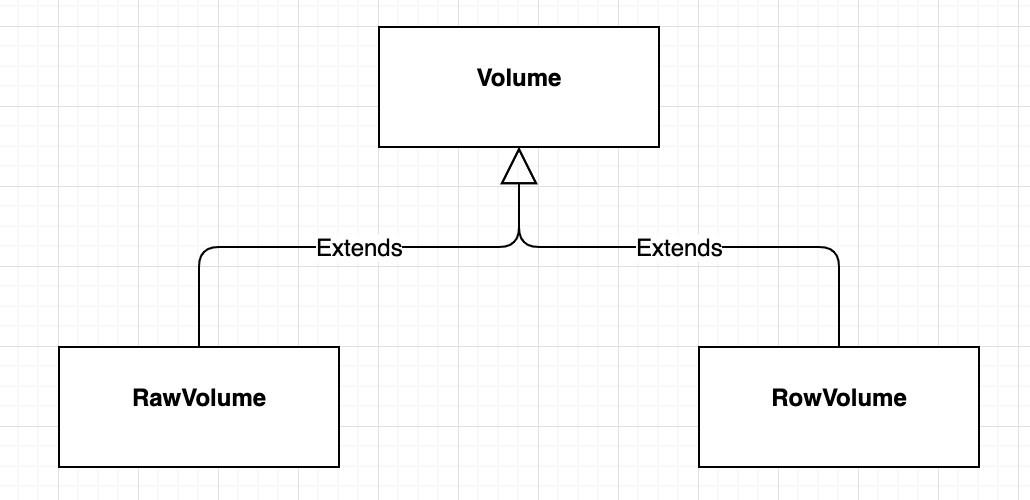
\includegraphics[width=10cm]{../imgs/volume-type.png}
\end{center}

\section{ROW}

想象有一日志系统(CDP),快照就是日志系统里的时间点。
当前卷的状态依赖于前面的日志记录。

ROW与此类似,删除快照实现复杂,同时需要优化读性能。

ROW设计问题
\begin{enumbox}
\item 链式快照和树状快照
\item 平安需求:可写快照?
\item ***
\item 卷和快照的关系,是共存于一个物理卷、还是各自独立构成一个物理卷。若独立占有一个物理卷,则打快照后,会改变卷ID,凡是依赖于这个信息的地方都需要进行适配。
\item 在哪一层实现ROW
\item 索引的page cache
\item 跨卷读,clone
\item 读取需要合并多个快照上的数据块。建立全量索引及其cache可以加速这一过程。
\item 快照头的映射表如何组织?是全索引,还是增量索引?
\item ROW读快照和读卷是同一个过程?
%\item COW里卷上有完整数据,快照有增量数据。
%\item ROW第一次快照有全量数据,后续快照和卷无完整数据。ROW很自然地体现了增量过程。
\end{enumbox}

\section{操作}

\subsection{create}

\begin{center}
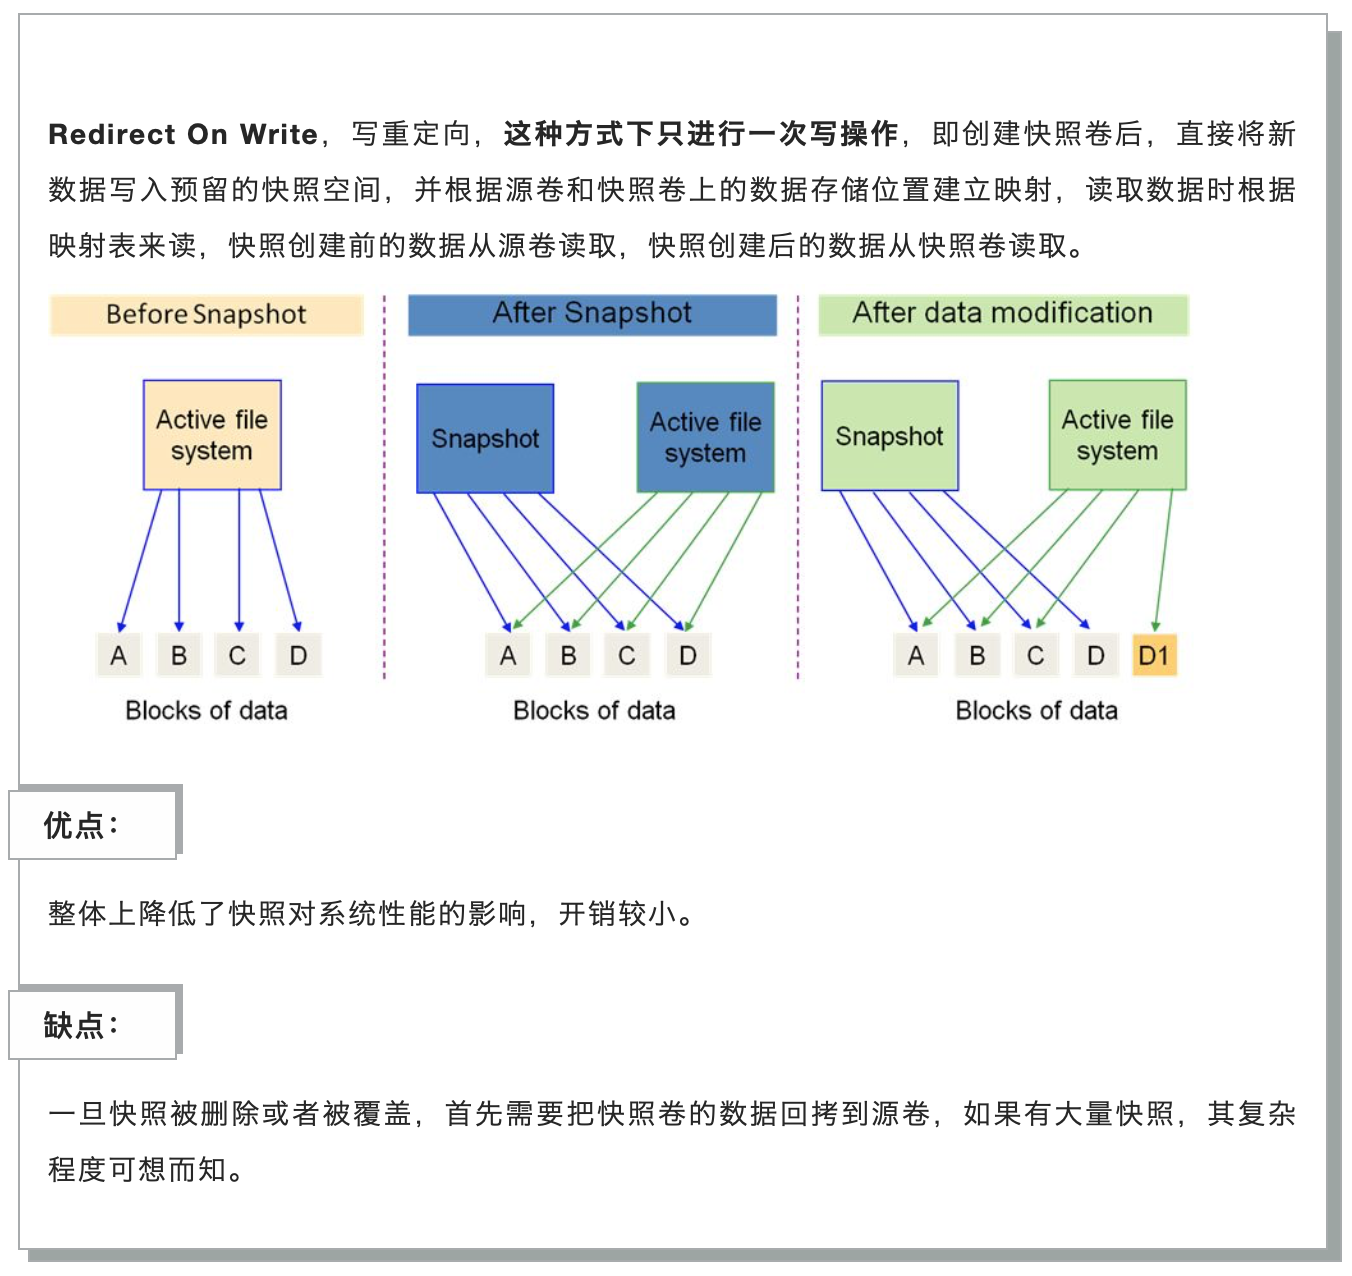
\includegraphics[height=10cm]{../imgs/snapshot/row-snapshot.png}
\end{center}

如果发生卷ID变化,上层应用需要重新打开卷,影响较大。

用户通过命令行创建快照,卷的描述符应有快照方面的信息。

创建快照是通过哪个leader执行的?

从leader方面看,client端与rangectl都需要快照树的结构信息,怎么在多个节点之间进行同步?
加入version,每个holder维护该属性,消息中也携带该属性,如果发现过期,则做相应处理。

如果有多个client端,如何一一通知到呢?

\subsection{delete}

\begin{center}
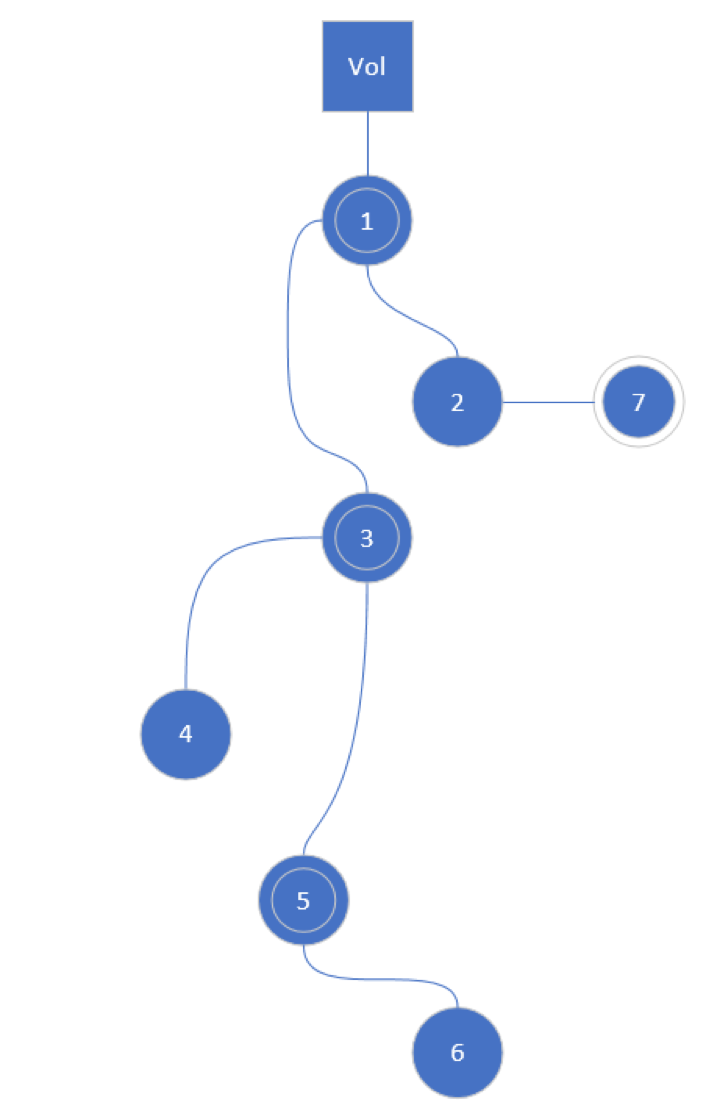
\includegraphics[height=10cm]{../imgs/snapshot/snaptree.png}
\end{center}

快照包含有增量数据,除了叶子快照,不能直接删除。
\begin{enumbox}
\item 根节点,不可删除,只有当快照节点仅剩本节点,并且发生回滚时删除,卷回到无快照状态
\item 快照中间节点
\item 快照中间节点
\item 快照叶子节点
\item 快照中间节点
\item 快照叶子节点
\item 卷所在位置,随着回滚在各个快照上漂移。
\end{enumbox}

空间回收策略
\begin{enumbox}
\item 叶子节点删除,可以完全回收在该时刻之后分配的空间
\item 中间节点,比如3,删除后其实还存在,当子节点删除后自动删除,因此在真正删除前并不能回收空间;
\item \hl{同时,当1上没有其他子节点时,可以做向上合并}。
\end{enumbox}

\begin{center}
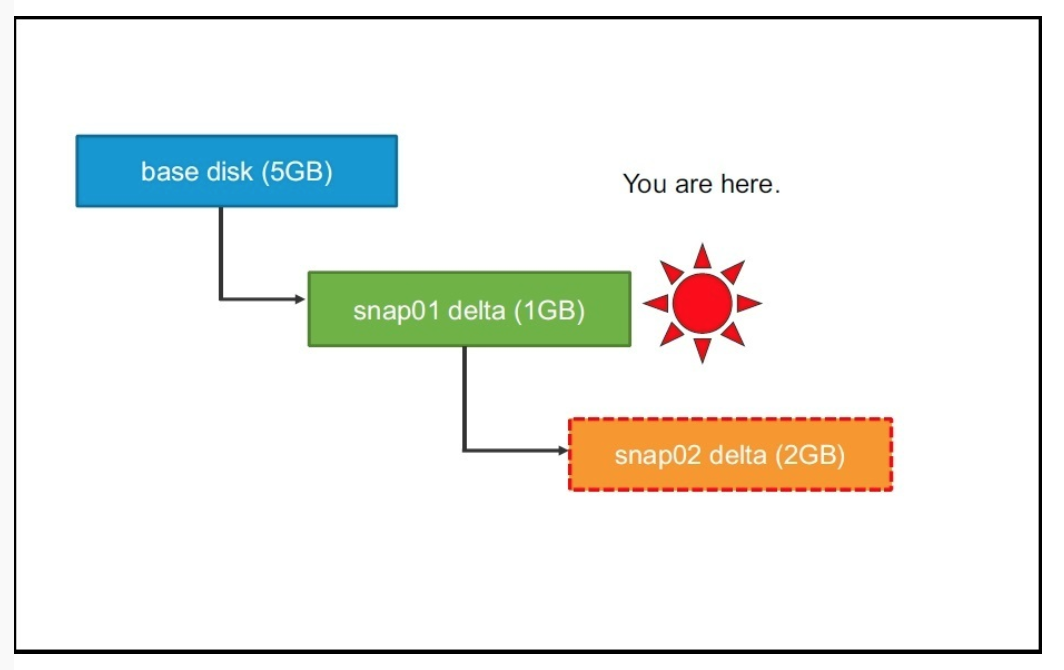
\includegraphics[width=10cm]{../imgs/snapshot/snap-delete-leaf.png}
\end{center}

\begin{center}
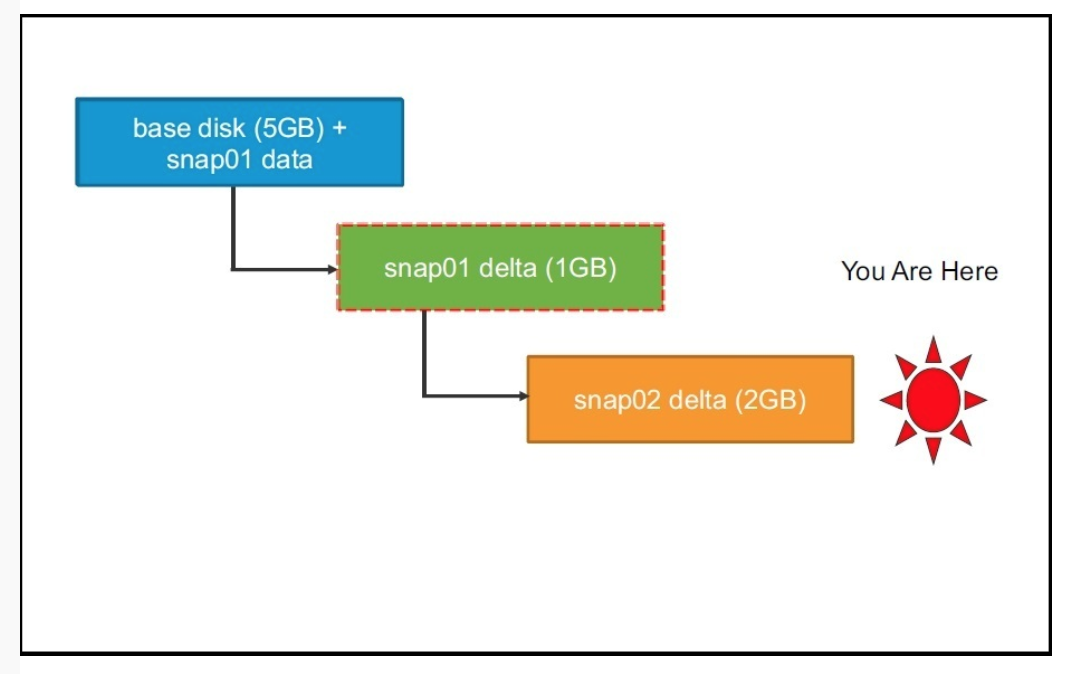
\includegraphics[width=10cm]{../imgs/snapshot/snap-delete-non-leaf.png}
\end{center}


\subsection{rollback}

直接用目标快照的快照头替换卷的快照头。

回收卷私有数据

\subsection{list}

快照树,隐藏或显示删除的快照。

\subsection{read}

\subsection{clone}

读取snapshot的内容。读取卷和快照是同一个过程。

\begin{center}
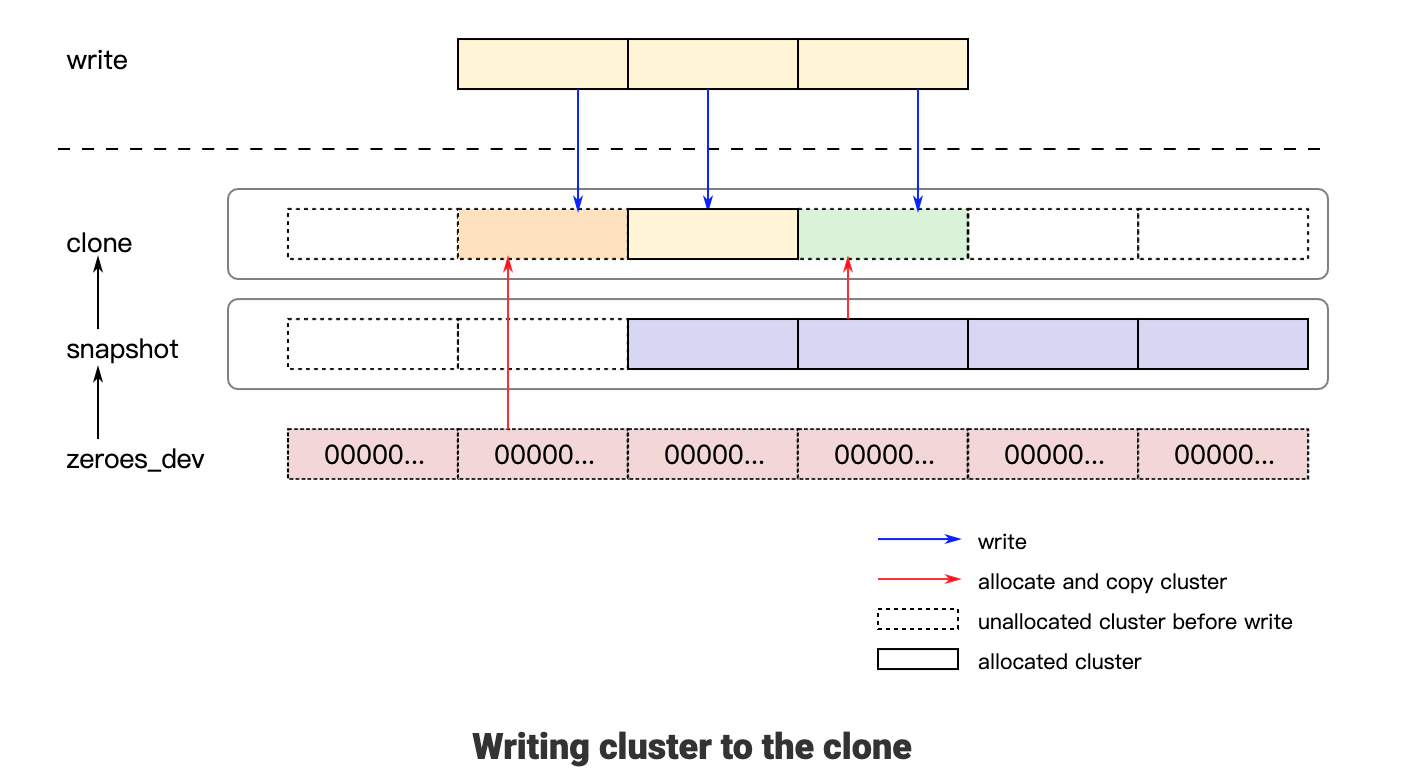
\includegraphics[width=10cm]{../imgs/snapshot/clone-write.png}
\end{center}

\begin{center}
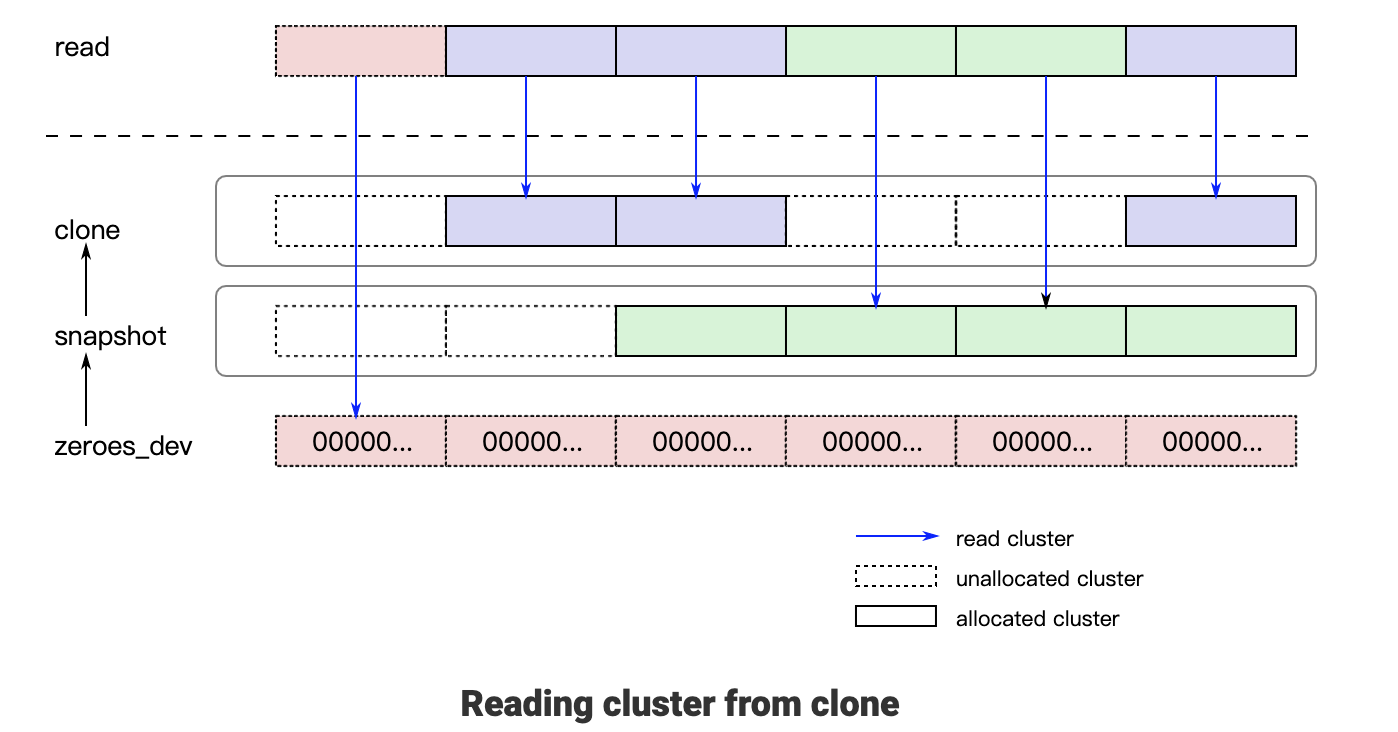
\includegraphics[width=10cm]{../imgs/snapshot/clone-read.png}
\end{center}

\subsection{flatten}

\subsection{protect/unprotect}

\section{实现}

\subsection{引入VolumeCtl}

创建、删除等快照操作通过VolumeCtl进行。

\hl{创建和删除快照操作是卷级操作}。如快照树结构发生变化,当如何?
LICH中快照树的变化和访问都是通过卷控做得,所以没有一致性问题。
suzaku中client端充当卷控角色,在多活的情况下,有什么影响?

% 因为快照是只读的,是否可以简化实现?

\subsection{快照树}

一个卷的卷和所有快照构成单根树结构。相关信息持久化到ETCD上。包含指向快照元数据的\hl{chkidx列表}。

% 写IO涉及\hl{当前快照},读IO可能涉及多个快照。
% 快照读与读IO一致,可能涉及多个快照。

% IO的写和读都由client/target进行?在get token里返回物理地址。返回一个或多个token对象?

\subsection{单个快照}

\begin{center}
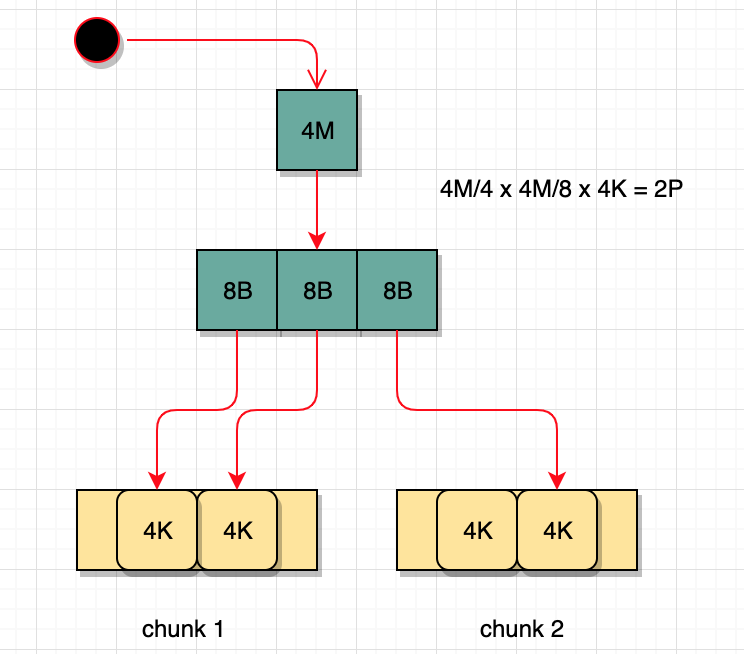
\includegraphics[width=10cm]{../imgs/snapshot/snapshot-head.png}
\end{center}

元数据映射表在哪里维护?与\hl{chunk-副本元数据}一样维护?
% 找get token里返回物理地址。client直接读写该地址。逻辑上连续,物理上未必连续。

% 每个range ctl也维护卷的所有快照的对应范围?按snap name进行索引?
% 当snaptree结构发生变化时,rangectl重新加载?
% 多活的场景下,会有什么问题吗?

如何表示页的物理地址:
\begin{center}
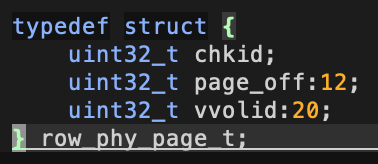
\includegraphics[width=10cm]{../imgs/snapshot/row-phy-page.png}
\end{center}

\subsection{虚拟卷和物理卷的关系}

一种表示法:导出不变的虚拟卷,虚拟卷可以包含多个物理卷,一个快照对应一个物理卷。

另一种表示法:用一个物理卷包含虚拟卷及其快照。

\subsection{Volume Allocator}

封装底层物理卷的访问接口。可以运行在任意backing store上,如file、LUN。

特性:
\begin{enumbox}
\item 引入资源池
\end{enumbox}

优化碎片化的措施:
\begin{enumbox}
\item 事前
\item 事后
\end{enumbox}

\subsection{地址映射}

加入v2p过程:
\begin{center}
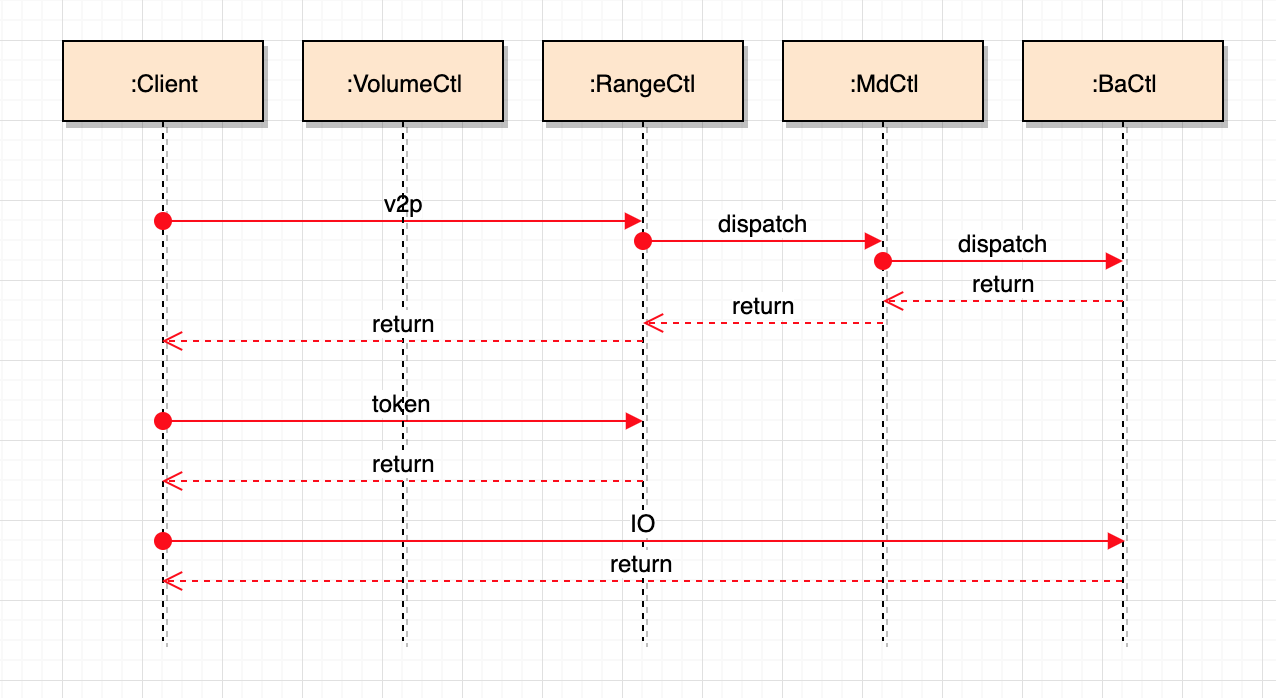
\includegraphics[width=10cm]{../imgs/data-path.png}
\end{center}

\section{参考产品}

\begin{enumbox}
\item SheepDog/SSAN
\item Open VStorage
\item ***
\item FusionSorage
\item NetApp WALFS
\item Dell SC Series
\item 阿里云ECS
\item ***
\item SPDK
\item QEMU qcow2
\end{enumbox}
